Введём понятие функционала. $y = f(x)$ --- отображение числового множества $r \in X$ на числовое множество $y \in Y$ --- функция. $X$ --- конечномерное множество
\begin{equation}
	\mathrm{I} [y(x)] = \int\limits_a^b F(x, y(x), y'(x))\,dx
	\label{equ:Variz1}
\end{equation}
Функционал \eqref{equ:Variz1} отображает множество функций на числовое множество. Множество функций является областью определения.\\

\textbf{Задача Бернулли}\\
\begin{figure}[h!]
	\centering
	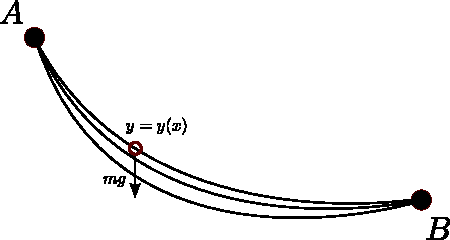
\includegraphics{figVariaz.pdf}
\end{figure}

Требуется найти кривую $y(x)$, чтобы шарик попал из ($\cdot$)$A$ в ($\cdot$)$B$ c наименьшей скоростью
\[
	t = \int\limits_a^b  \frac{\sqrt{1 + y'^2}}{\sqrt{2 g y}}\, dx
\]

Найдо найти экстремум функционала $\mathrm{I}[y(x)]$ на множестве непрерывно дифференциируемых функций: $y(x) \in C_1$.
Предположим, что искомая кривая --- прямая, соединяющая $A$ и $B$
\begin{wrapfigure}{r}{0.4\textwidth}
	\centering
	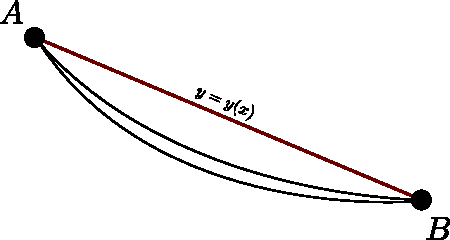
\includegraphics[width=0.4\textwidth]{figVariaz2.pdf}
\end{wrapfigure}
Рассмотрим множество кривых. Их можно описать уравнением
\[
	\tilde y (x, \alpha) = y (x) + \alpha\eta(x), \quad 0 \leqslant \alpha \leqslant 1.
\]
\[
	\eta \in C_1 \qquad \eta(a) = \eta(B) = 0
\]
Необходимо рассмотреть функционал на однопараметрическом семействе кривых:
\[
	\mathrm{I}[\tilde y (x, \alpha)] = \int\limits_a^b F(x, \tilde y(x, \alpha), \tilde y'(x, \alpha)) \, dx
\]
Искомая кривая будет получаться при $\alpha = 0$. Предположим нам удалось взять интеграл в аналитическом виде, когда $x$ у нас пропадает и получаем функцию зависящую только от $\alpha$:
\[
	\tilde{\mathrm{I}}(\alpha)
\]
Необходимое условие экстремума функционала:
\[
	\delta \mathrm{I} = \lim\limits_{\alpha \to 0} \derp{\tilde{\mathrm{I}}}{\alpha}{} = 0 
\]
--- \textit{первая вариации функционала}.
\[
	\derp{\tilde{\mathrm{I}}}{\alpha}{} = \int\limits_a^b \left(\derp{F}{\tilde y}{} \derp{\tilde y}{\alpha}{} + \derp{F}{\tilde y}{} \derp{\tilde y'}{\alpha}{} \right)\, dx
\]
\[
	\derp{\tilde y}{\alpha}{} = \eta (x) \qquad \derp{\tilde y '}{\alpha}{} = \eta' (x)
\]
Таким образом 
\[
	\derp{\tilde{\mathrm{I}}}{\alpha}{} = \int\limits_a^b \left(\derp{F}{\tilde y}{} \eta (x) + \derp{F}{\tilde y}{} \eta'(x)\right)\, dx.
\]
Переходим к пределу, чтобы получить первую вариацию:
\[
	\delta \mathrm{I} \lim\limits_{\alpha \to 0} \derp{\tilde{\mathrm{I}}}{\alpha}{} = \int\limits_a^b \left(\derp{F}{y}{} \eta(x) + \derp{F}{y}{} \eta'(x)\right)\, = 0
\]
\[
	\int\limits_a^b \derp{F}{y}{} \eta(x)\, dx + \derp{F}{y'}{} \eta(x) \Big|_a^b - \int\limits_a^b \der{}{x}{} \derp{F}{y'}{} \eta(x)\, dx = 0
\]
На концах отрезка произвольная функция обращается в 0.
\[
	\delta I = \int\limits_a^b \left(\derp{F}{y}{} - \der{}{x}{} \derp{F}{y'}{} \right) \eta(x)\, dx = 0
\]
Так как $\eta(x)$ --- произвольная, то $\int = 0$ только в случае, когда выражение в скобках $= 0$\\

Окончательное условие для функционала записывается в виде уравнения Эйлера:
\[
	\der{}{x}{} \derp{F}{y'}{} - \derp{F}{y}{} = 0
\]


\subsubsection{Вариационная задача с кратным интегралом.}
Возьмём на плоскости $xOy$ область $D$ и на ней построим цилиндр, покрытый поверхностью $z = \varphi(x, y)$:
\begin{wrapfigure}[3]{l}{0.35\textwidth}
	\centering
	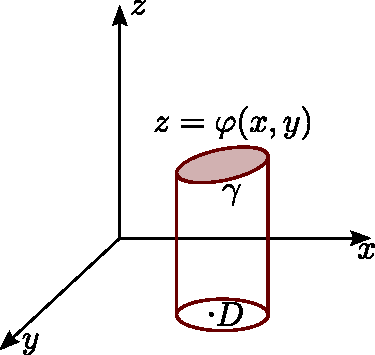
\includegraphics[width=0.35\textwidth]{figVariaz3.pdf}
\end{wrapfigure}
\begin{align*}
	&\mathrm{I} [\varphi(x, y)] = \iint\limits_S F(x, y, \varphi(x, y), \derp{\varphi}{x}{}, \derp{\varphi}{y}{})\, dx dy +{} \\
	&\phantom{\mathrm{I} [\varphi(x, y)]=} + \int\limits_\gamma G(\varphi(x, y), \varphi'(x, y))\, d\gamma =\\
	&\phantom{\mathrm{I} [\varphi(x, y)]} = \int\limits_D \left(\left(\derp{\varphi}{x}{} \right)^2 + \left(\derp{\varphi}{y}{} \right)^2 - c \varphi^2 - 2 f \varphi\right)\, dx dy + {}\\
	&\phantom{\mathrm{I} [\varphi(x, y)]=} + \int\limits_\gamma \left(\sigma \varphi^2 - c \varphi \right)\, d \gamma
\end{align*}\\

Мы должны рассмотреть однопараметрическое семейство плоскостей:
\[
	\tilde \varphi(x, y) = \varphi (x ,y) + \alpha \eta (x, y),
\]
выходящих из контура $\gamma$: $r \big|_\gamma = 0$


\begin{multline*}
	\mathrm{I} [\tilde \varphi(x, y)] = \iint\limits_S \left\{\left[ \derp{}{x}{} (\varphi + \alpha r) \right]^2 + \left[\varphi + \alpha r \right]^2  - c [\varphi + \alpha r]^2 - 2 f (\varphi + \alpha r)\right\}\, dx dy  +{}
	\\+ \int\limits_\gamma \left[ \sigma (\varphi + \alpha r)^2 - c (\varphi + \alpha r) \right]\, d\gamma = \\
	= \iint\limits_S \left\{\left(\derp{\varphi}{x}{} + \alpha \derp{r}{x}{} \right)^2 + \left(\derp{\varphi}{y}{} + \alpha \derp{r}{y}{}\right) - c (\varphi + \alpha r)^2 - 2 f (\varphi + \alpha r)\right\}\, dx dy +{}
	\\+ \int\limits_\gamma \left[\sigma (\varphi + \alpha r)^2 - c (\varphi + \alpha r) \right]\, d\gamma
\end{multline*}
\begin{multline*}
	\derp{I}{\alpha}{} \iint\limits_D \left\{ 2 \left[\derp{\varphi}{x}{} + \alpha \derp{r}{x}{} \right] \derp{r}{x}{} + 2 \left(\derp{\varphi}{y}{} + \alpha \derp{r}{y}{} \right) \derp{r}{y}{}  - 2 c (\varphi + \alpha r) r - 2 f r \right\}\, dx dy +{}\\
	+ \int\limits_\gamma \left\{2 \left[\sigma \left(\varphi + \alpha r \right)r \right] - c r\right\}\, d \gamma
\end{multline*}
\[
	\delta \mathrm{I} = \lim\limits_{\alpha \to 0} \derp{\tilde{\mathrm{I}}}{\alpha}{} = 2 \iint\limits_D \left\{ \derp{\varphi}{x}{} \derp{r}{x}{} + \derp{\varphi}{y}{} \derp{r}{y}{} - c \varphi - f r \right\}\, dx dt + \int\limits_\gamma (2 \sigma \varphi r - c r)\, d \gamma = 0
\]
\[
	\delta \mathrm{I} = 2 \iint\limits_D \left\{\derp{}{x}{} \left[\derp{\varphi}{x}{} r \right] - \derp{\varphi}{x}{2} r + \derp{}{y}{} \left(\derp{\varphi}{y}{} r \right) - \derp{\varphi}{y}{2} r - c \varphi r - f r\right\}\, dx dy =
	\int\limits_\gamma \left[ w \sigma \varphi r - c r \right]\, d\gamma
\]
\begin{multline*}
	\iint\limits_D \left[\derp{}{x}{} \left( \derp{\varphi}{x}{} r \right) + \derp{}{y}{} \left( \derp{\varphi}{y}{} \right) r \right]\, dx dy 
	= \int\limits_\gamma \left[ \derp{\varphi}{x}{} r \cos (n x) + \left(\derp{\varphi}{y}{} r \right) \cos (n y) \right]\, d\gamma=\\
	= \int\limits_\gamma \overrightarrow{\mathrm{grad} \varphi} \vec n r\, d\gamma = \int\limits_\gamma \derp{\varphi}{n}{} r\, d\gamma
\end{multline*}
\[
	\delta \mathrm{I} = 2 \iint\limits_D \left[- \left(\derp{\varphi}{x}{} + \derp{\varphi}{y}{2}\right) - c \varphi - f \right] r \, dx dy + \int\limits_\gamma (2 \sigma \varphi - c + 2 \derp{\varphi}{n}{}) r \, d\gamma = 0
\]

\subsubsection{Вариационная формулировка задач}
Третья краевая задача для уравнения эллиптического типа:
\[
	\begin{cases}
		\displaystyle\derp{\varphi}{x}{2} + \derp{\varphi}{y}{} + c \varphi - f = 0\\
		\displaystyle\derp{\varphi}{n}{} + \sigma \varphi - \frac{c}{2} = 0 \Big|_\Gamma
	\end{cases}
\]
Решить краевую задачу и минимизировать функционал
\[
	\mathrm{I} [\varphi(x, y)] = \iint\limits_D \left\{\left(\derp{\varphi}{x}{} \right)^2 + \left(\derp{\varphi}{y}{} \right)^2 - c \varphi^2 - 2 f \varphi \right\}\, dx dy + \int\limits_\gamma \left(\sigma \varphi^2 - c \varphi\right)\, d\gamma
\]
\[
	\derp{u}{x}{2} + \derp{u}{y}{2} = - 1
\]
\[
	\abs{x} \leqslant 1 \qquad \abs{y} \leqslant 1
\]
\[
	u\big|_\gamma = 0
\]
Задача Дирихле для уравнения Пуассона
\[
		\mathrm{I} [\varphi(x, y)] = \iint\limits_D \left\{\left(\derp{\varphi}{x}{} \right)^2 + \left(\derp{\varphi}{y}{} \right)^2  - 2 u \right\}\, dx dy 
\]
